%!TEX root = ../../thesis.tex
\define{\chapterpath}{\allchapterspath/bci}
\define{\imgpath}{\chapterpath/img}

\define{\plotsize}{0.6}
\define{\sequencesize}{1}

\chapter{Application to Brain Computer Interaction}
\label{chapter:bci}
\minitoc


We have presented an algorithm that exploits task constraints to solve simultaneously a task under human feedback and learn the associated meanings of the feedback signals. We have detailed an uncertainty measure than allow our agent to solve this problem more efficiently and shown that our algorithm can transition from task to task in a smooth way. This has important practical application since the user can start controlling a device from scratch, without the need of an expert to define the meaning of signals or carrying out a calibration phase. 

In this section, we explore the use of our algorithm to the brain computer interaction following the same reaching task scenario as presented in chapter~\ref{chapter:planning:method}. After discussing the related work, we will first test our algorithm with a database of EEG signals and compare its performance with a calibration procedure method that first collect known signal-label pair and train a unique classifier. We will present one experiment in more details and show that our algorithm conserve good properties on EEG signals and has important advantage over calibration based method. 

However we will point out a main difference between calibration procedure and our self-calibration method in that the EEG signals properties can be affected by the action of the agent. As our planning method can not guarantee the same agent behavior than during the calibration procedure, the quality of the signal received by the users can be impacted. To address this problem we will introduce a prior information of the Error-related potential EEG signals used, namely that the signal corresponding to an ``incorrect'' meaning are more ``powerful'' than the one associated to meaning ``correct''. We will exploit this properties, in addition to our interpretation hypothesis method, and show that we can achieve better performances. We finally present results where different users teach an agent to reach a particular state by assessing the agent action in their mind, and without calibrating the system before hand.

Those results with real EEG signals allow us to believe such algorithm could have practical application into the real word. By removing the user of an expert to collect and calibrate the system, we may democratize the use of brain computer interface and allow their users to go out of the labs. However there is number of limitation that would need to be addressed, such as the synchronous interactions assumption, the discrete state, discrete action. Most of the current limitation of this work will be addressed in the next section.

The application of this work to BCI is a collaboration with I{\~n}aki Iturrate and Luis Montesano.

%%%%%%%%%%%%%%%%%%%%%%%%%%%%%%%%%%%%%%%%%%%%%%
%%%%%%%%%%%%%%%%%%%%%%%%%%%%%%%%%%%%%%%%%%%%%%
%%%%%%%%%%%%%%%%%%%%%%%%%%%%%%%%%%%%%%%%%%%%%%
%%%%%%%%%%%%%%%%%%%%%%%%%%%%%%%%%%%%%%%%%%%%%%
%%%%%%%%%%%%%%%%%%%%%%%%%%%%%%%%%%%%%%%%%%%%%%
\section{Related work}


%%%%%%%%%%%%%%%%%%%%%%%%%%%%%%%%%%%%%%%%%%%%%%
%%%%%%%%%%%%%%%%%%%%%%%%%%%%%%%%%%%%%%%%%%%%%%
%%%%%%%%%%%%%%%%%%%%%%%%%%%%%%%%%%%%%%%%%%%%%%
%%%%%%%%%%%%%%%%%%%%%%%%%%%%%%%%%%%%%%%%%%%%%%
%%%%%%%%%%%%%%%%%%%%%%%%%%%%%%%%%%%%%%%%%%%%%%
\section{Using pre-recorded EEG signals}

real ErrP datasets recorded from previous experiments \cite{iturrate2013task}.

\subsection{Dataset and scenario}

\paragraph{EEG datasets} Once the algorithm was evaluated with artificial datasets, we tested the feasibility of the proposed self-calibration approach using real ErrP datasets. The objective of this analysis is to study the scalability of our method to EEG data, which may have different properties than our artificial dataset. 

The EEG data were recorded in a previous study \cite{iturrate2013task} where participants monitored on a screen the execution of a task where a virtual device had to reach a given goal. The motion of the device could be correct (towards the goal) or erroneous (away from the goal). The subjects were asked to mentally assess the device movements as erroneous or non-erroneous. The EEG signals were recorded with a gTec system with 32 electrodes distributed according to an extended 10/20 international system with the ground on FPz and the reference on the left earlobe. The ErrP features were extracted from two fronto-central channels (FCz and Cz) within a time window of $[200,700]$ ms (being 0 ms the action onset of the agent) and downsampled to $32$ Hz. This leaded to a vector of $34$ features.

\paragraph{Comparison with calibration methods} In order to show the benefit of learning without explicit calibration, we compare our method with the standard supervised BCI calibration procedure. In this calibration procedure, which can last for up to 40 minutes, the experimenter needs to record enough data from the user from several offline runs, where the user is not controlling the agent but just passively assessing its actions. Following the literature on ErrPs \cite{chavarriaga2010learning,iturrate2013task} our training data will consist of 80 percent of positive examples (associated to a correct feedback) and 20 percent of negative examples (associated to an incorrect feedback). Our proposed algorithm is compared with different (but standard) sizes of calibration datasets: 200, 300 and 400 examples.

\subsection{One example detailed}
Figure~\ref{fig:sequence} shows one particular run of 500 steps comparing our self-calibration method with a calibration procedure of 400 steps. The two independent runs use as real EEG dataset with $80\%$ ten-fold classification accuracy. As our algorithm is operational from the first step, it can estimate the real task when sufficient evidence has been collected. On the other hand, a calibration approach collects signal-label pairs for a fixed number of steps and use the resulting classifier without updating it. This provokes that, during the calibration phase, no tasks can be learned, substantially delaying the user's online operation.

\begin{figure}[!ht]
\centering
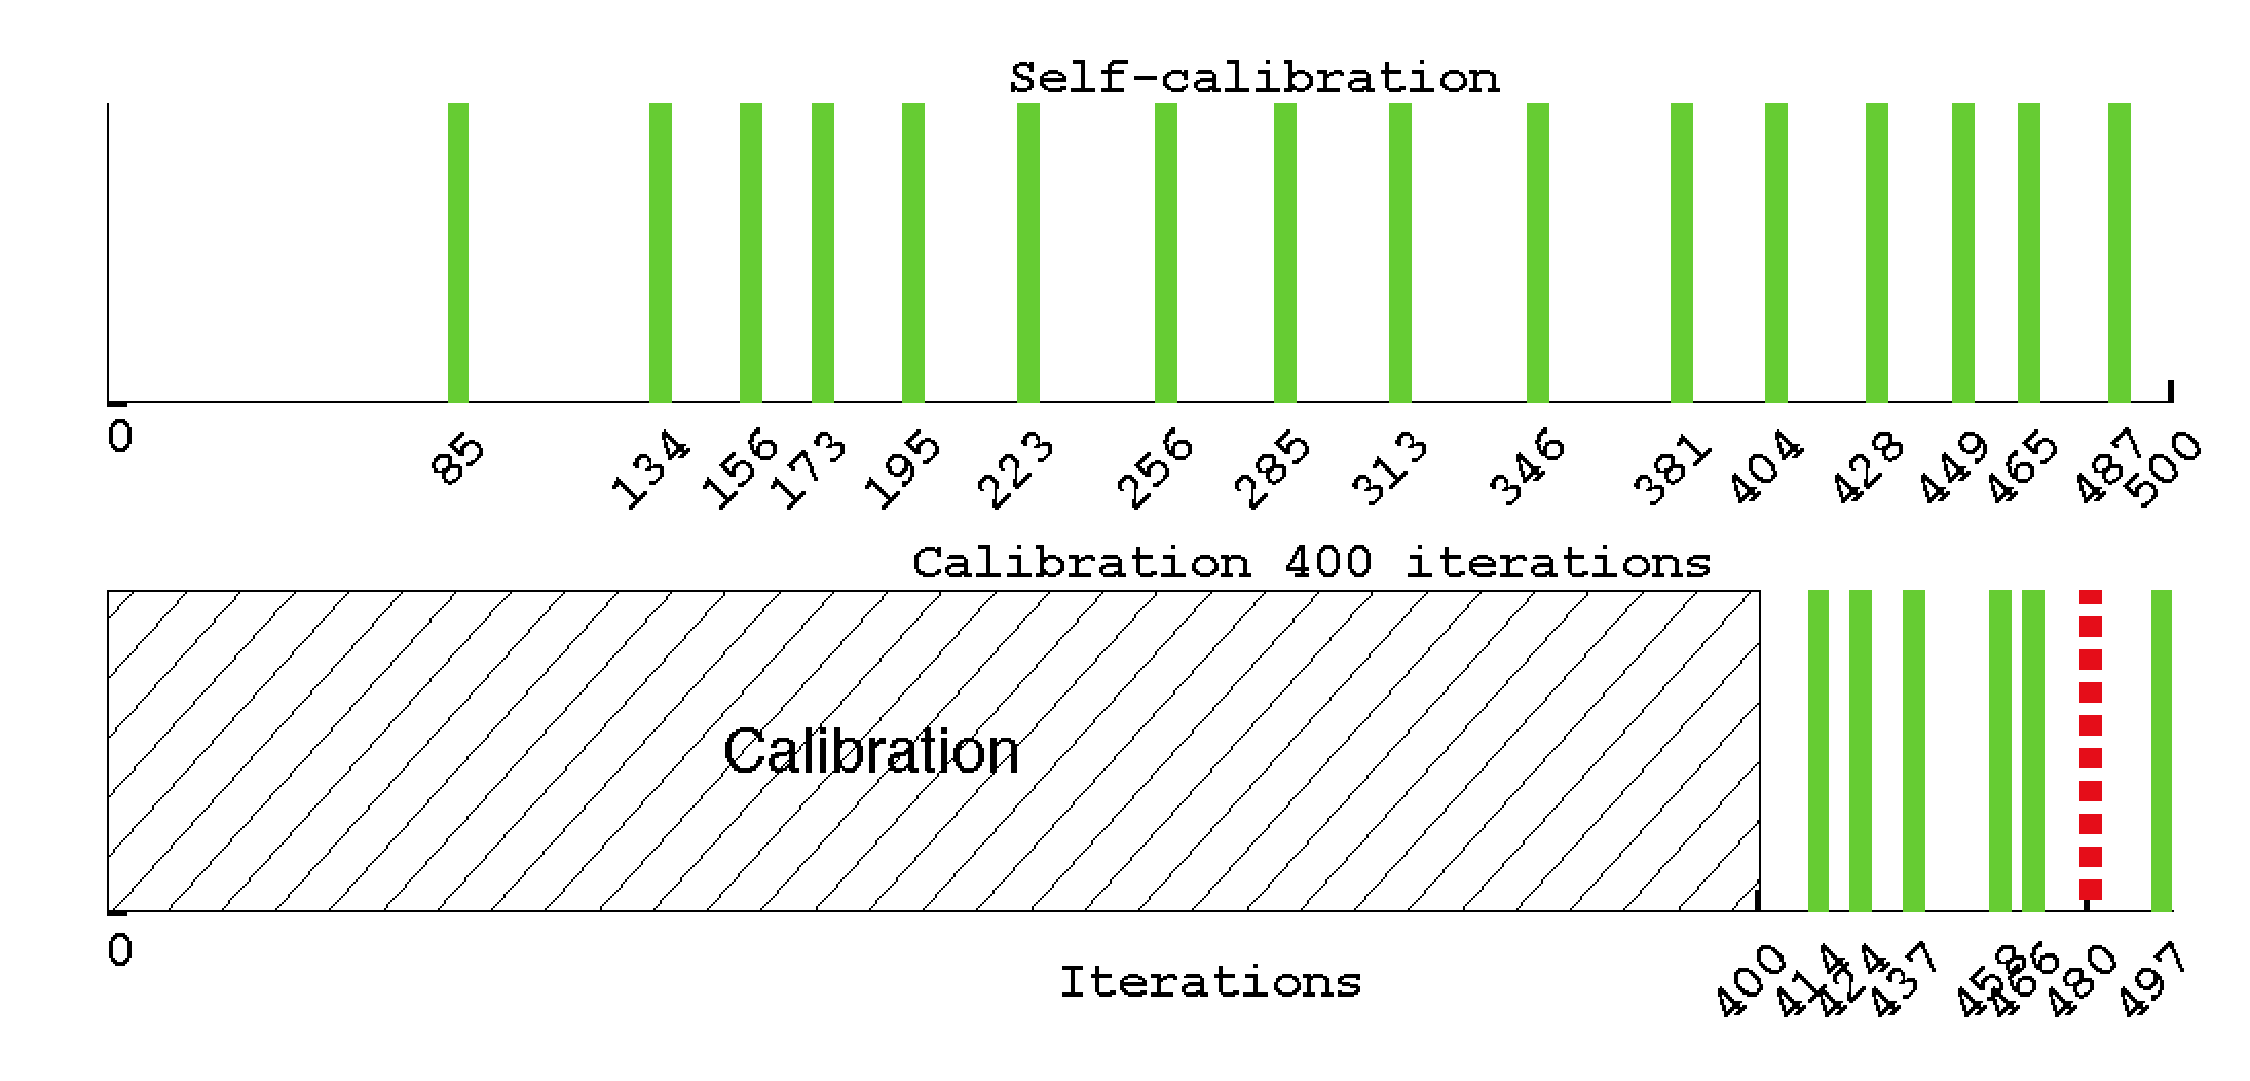
\includegraphics[width=\sequencesize\columnwidth]{\imgpath/plot_the_aaai_sequence.eps}
\caption{Time-line of one run from EEG dataset of $80$ percent ten-fold classification accuracy, self-calibration (top) versus 400 steps calibration (bottom). Green (filled) and red (dashed) bars represents respectively correct and incorrect task achievement. The proposed self-calibration method allow to reach a first task faster than would take a calibration procedure.}
\label{fig:sequence}
\end{figure} 



Figure~\ref{fig:sequence_evolution} shows the evolution of classification rate between our self-calibration method with a calibration procedure of 400 steps. As our method assigns different labels to each new teaching signal, the resulting classifiers have different performances, which help identifying the correct task. Once a task is identified (e.g.\ step 85 and 134), the corresponding labels are taken as ground truth, and all classifiers will have the same accuracies. As the agent starts exploring again to estimate the new tasks, all the classifiers except the true one will start to have worse accuracies again.

\begin{figure}[!ht]
\centering
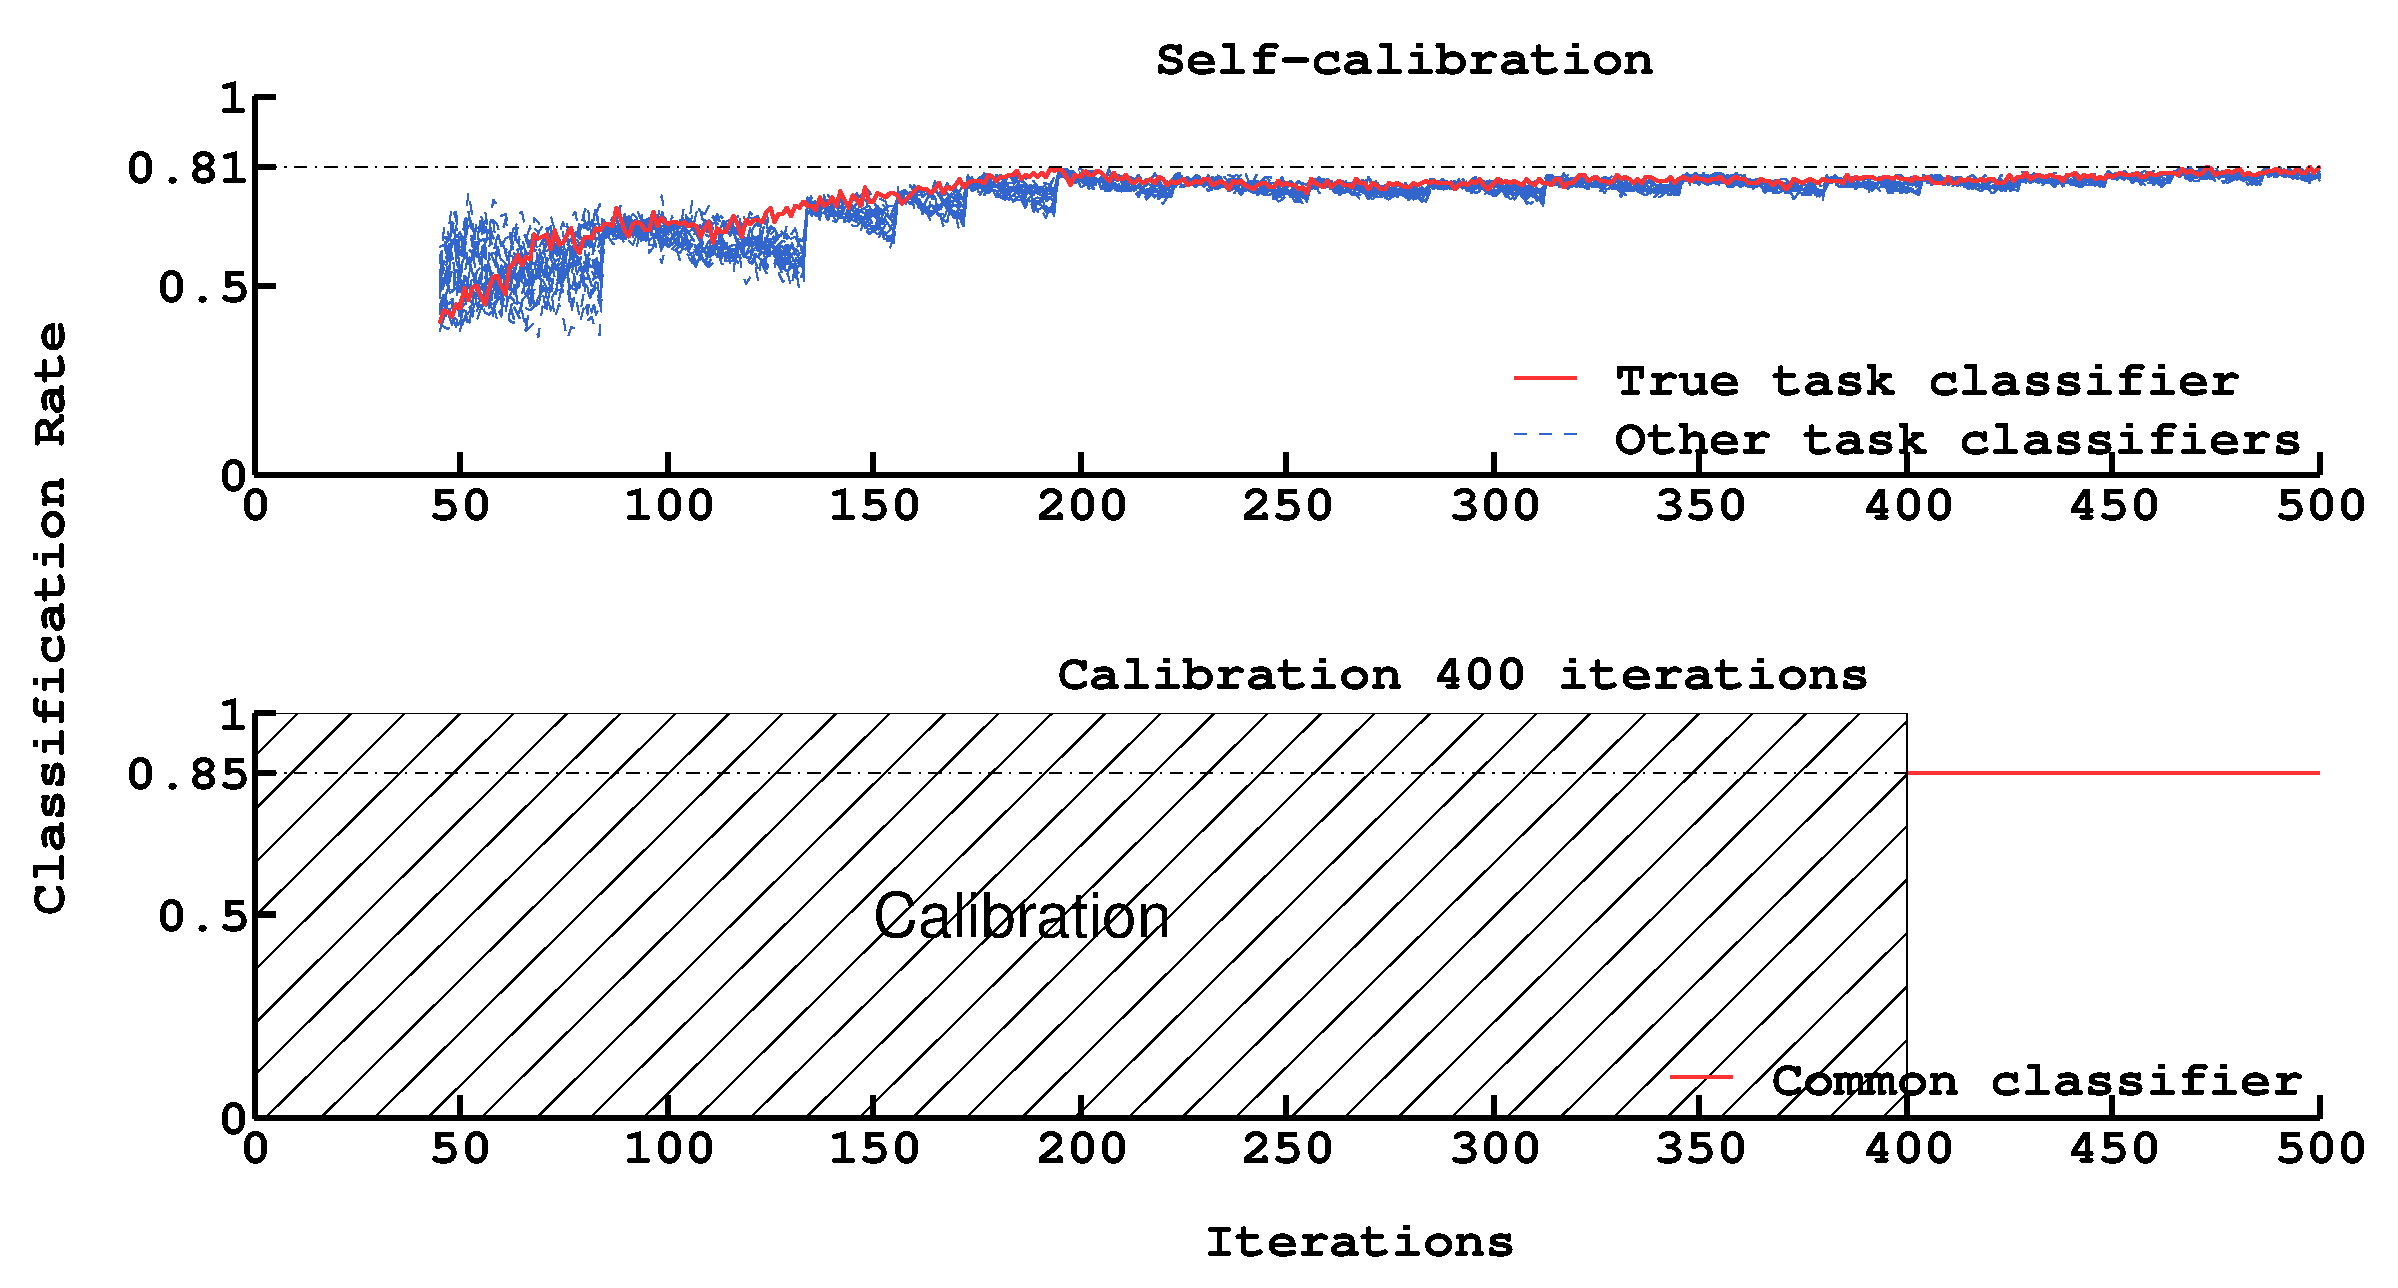
\includegraphics[width=\sequencesize\columnwidth]{\imgpath/plot_evo_classification_rate.eps}
\caption{Evolution of classification rate of one run from EEG data, self-calibration (top) versus 400 steps calibration (bottom). On top, the red line represents the classifier corresponding to the successive tasks taught by the user, the dashed blue lines represent all others tasks. Our method updates classifiers every steps.}
\label{fig:sequence_evolution}
\end{figure} 

\subsection{Planning}

\begin{figure}[!ht]
    \centering
    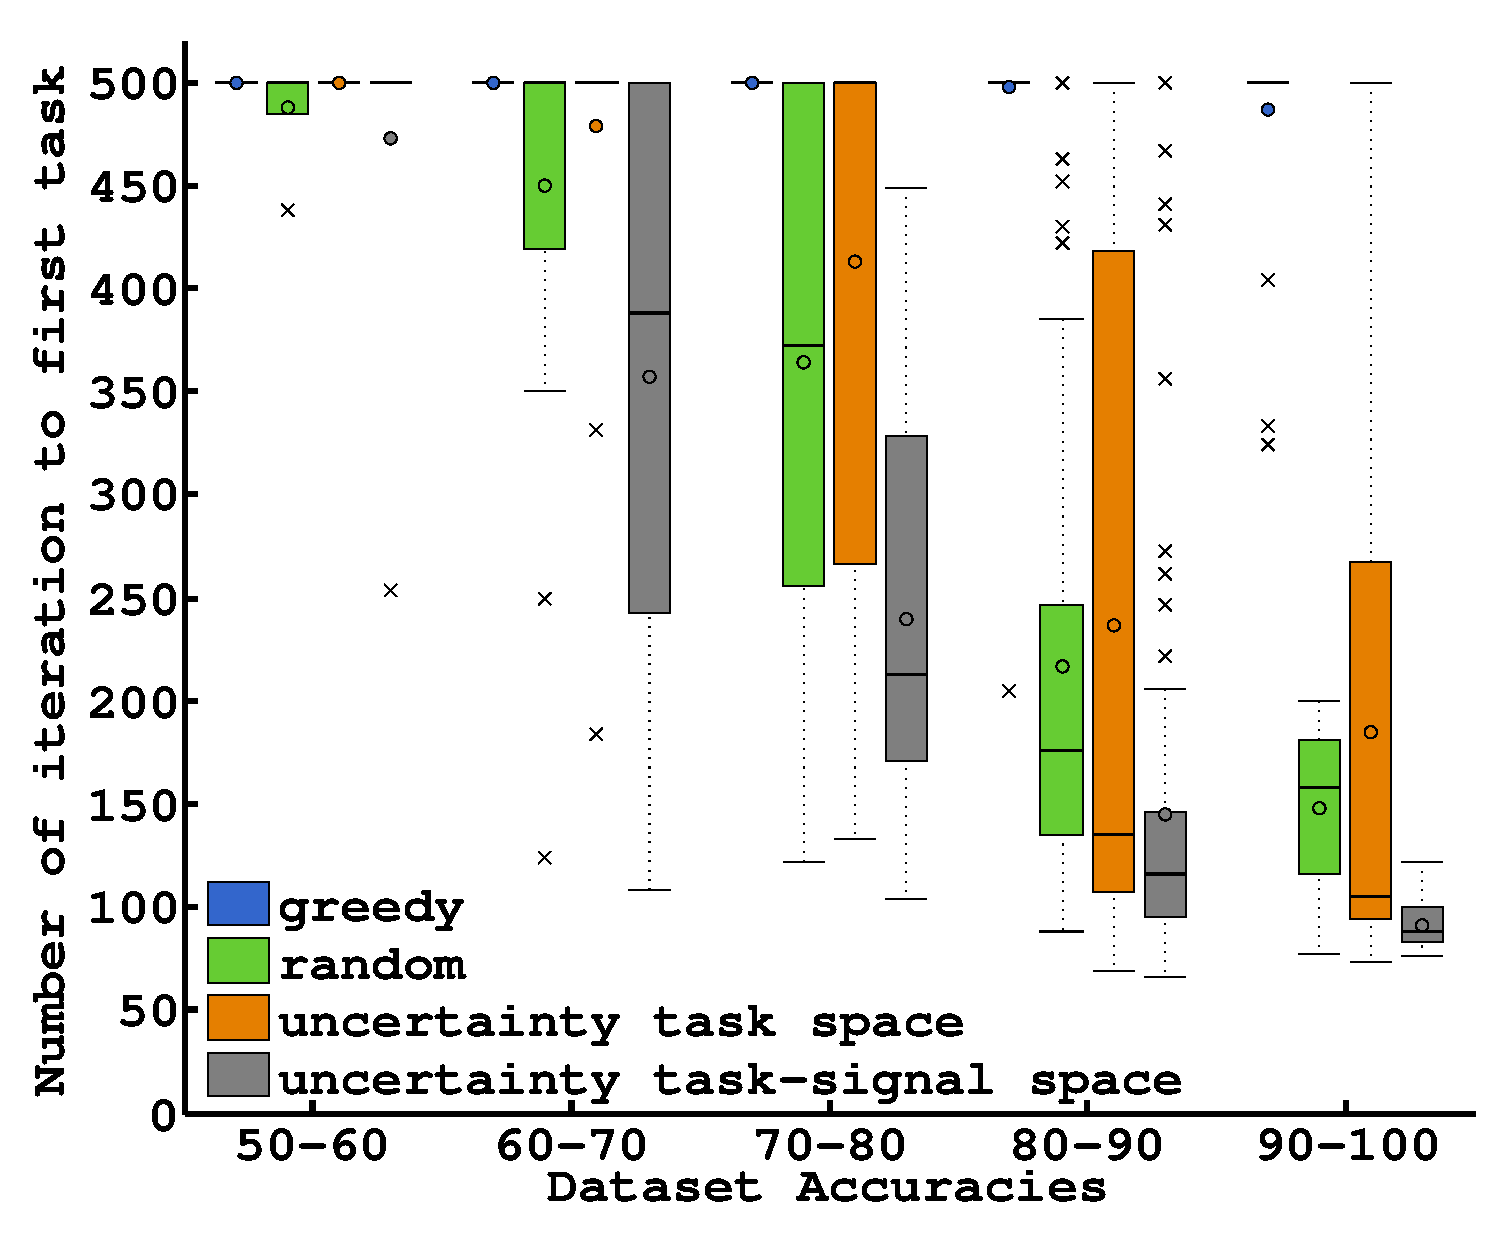
\includegraphics[width=\plotsize\columnwidth]{\imgpath/plot_EEG_planning.eps}
    \caption{Number of steps to complete first task using EEG data of different quality. The EEG data have similar properties than our 30 dimensional simulated data in Figure~\ref{fig:artificialplanning}. Our planning method based on both the task and the signal to meaning mapping uncertainty is more efficient that choosing action randomly, greedily or only based on the uncertainty on the task.}
    \label{fig:planningEEG}
\end{figure}


\subsection{Time to first task}

Figure~\ref{fig:firstEEG} shows the results per group of dataset. Our algorithm allows to complete the first task without errors and in a fair amount of iteration.  For our method, the learning time is strongly correlated with the dataset quality. However calibration methods, which do not update their classifier once calibrated, identify more tasks incorrectly.

\begin{figure}[!ht]
\centering
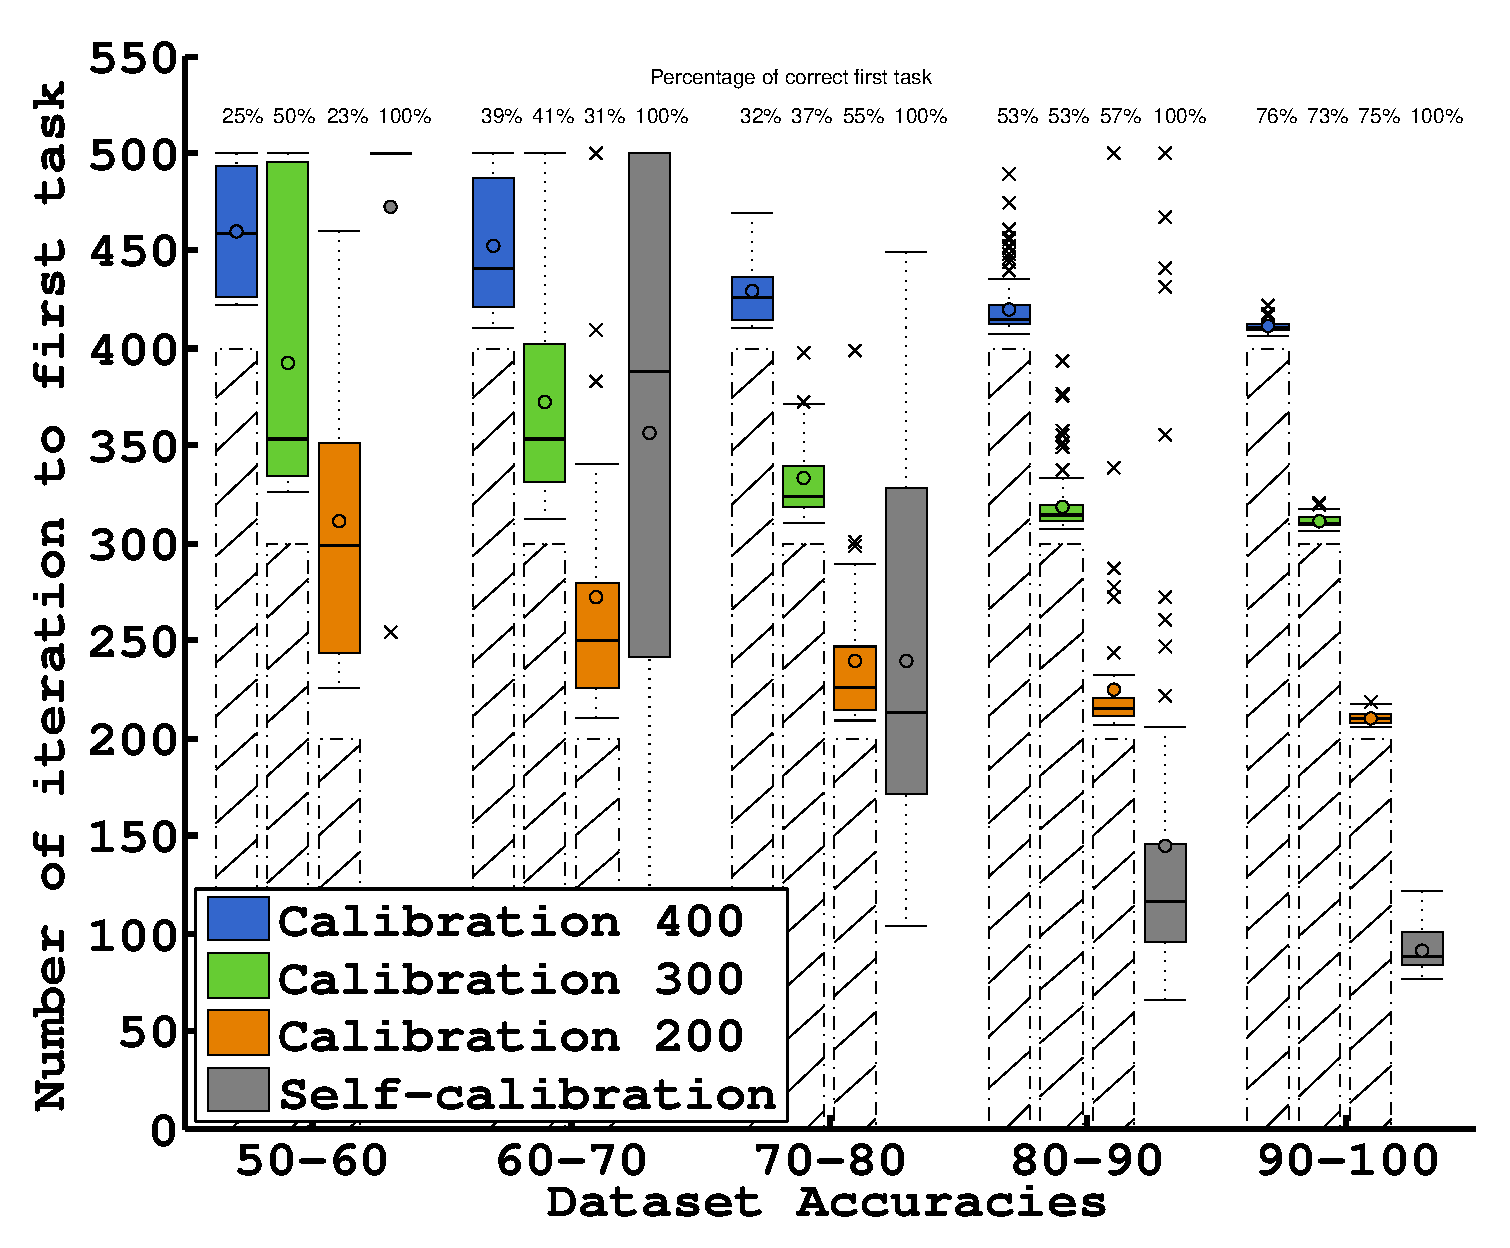
\includegraphics[width=\plotsize\columnwidth]{\imgpath/plot_EEG_calib_firstconf.eps}
\caption{Number of steps to complete first task with EEG data. The percentage of time the task first task was correct is show on top of the each box plot. The method scale well to EEG data. Contrary to the standard calibration approaches, we do not make mistakes with low quality datasets.}
\label{fig:firstEEG}
\end{figure} 

\subsection{Cumulative performances}

Figure~\ref{fig:nCorrectEEG} compares the number of tasks that can be achieved in 500 steps. With 90\% and more dataset quality we can achieve about 20 tasks on average. The results are consistent with artificial dataset analysis.

\begin{figure}[!ht]
\centering
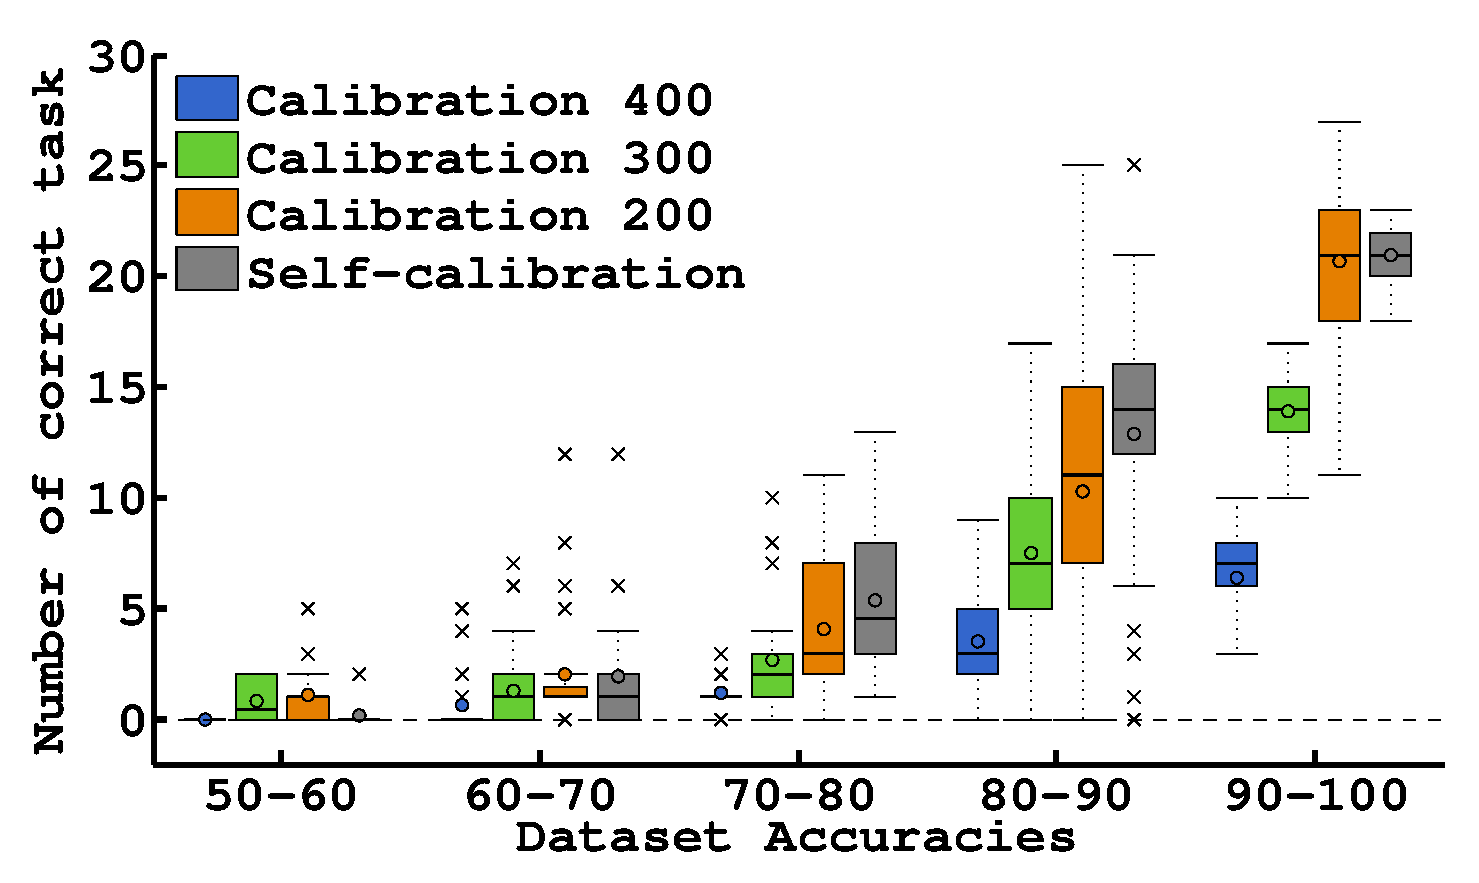
\includegraphics[width=\plotsize\columnwidth]{\imgpath/plot_EEG_calib_nCorrect.eps}
\caption{Number of task correctly achieved in 500 steps with EEG data. Calibration methods can not complete a significant number of task as most of the time is spent on calibration.}
\label{fig:nCorrectEEG}
\end{figure} 

The calibration methods can not complete many task as a significant amount of iteration was used for calibrating the system. A calibration of 200 steps makes as many good estimation than our method, but it also makes many wrong estimation, see Figure~\ref{fig:nWrongEEG}. For calibration methods, the less time spent on calibration, the poorer the classifier which implies more mistakes.

\begin{figure}[!ht]
\centering
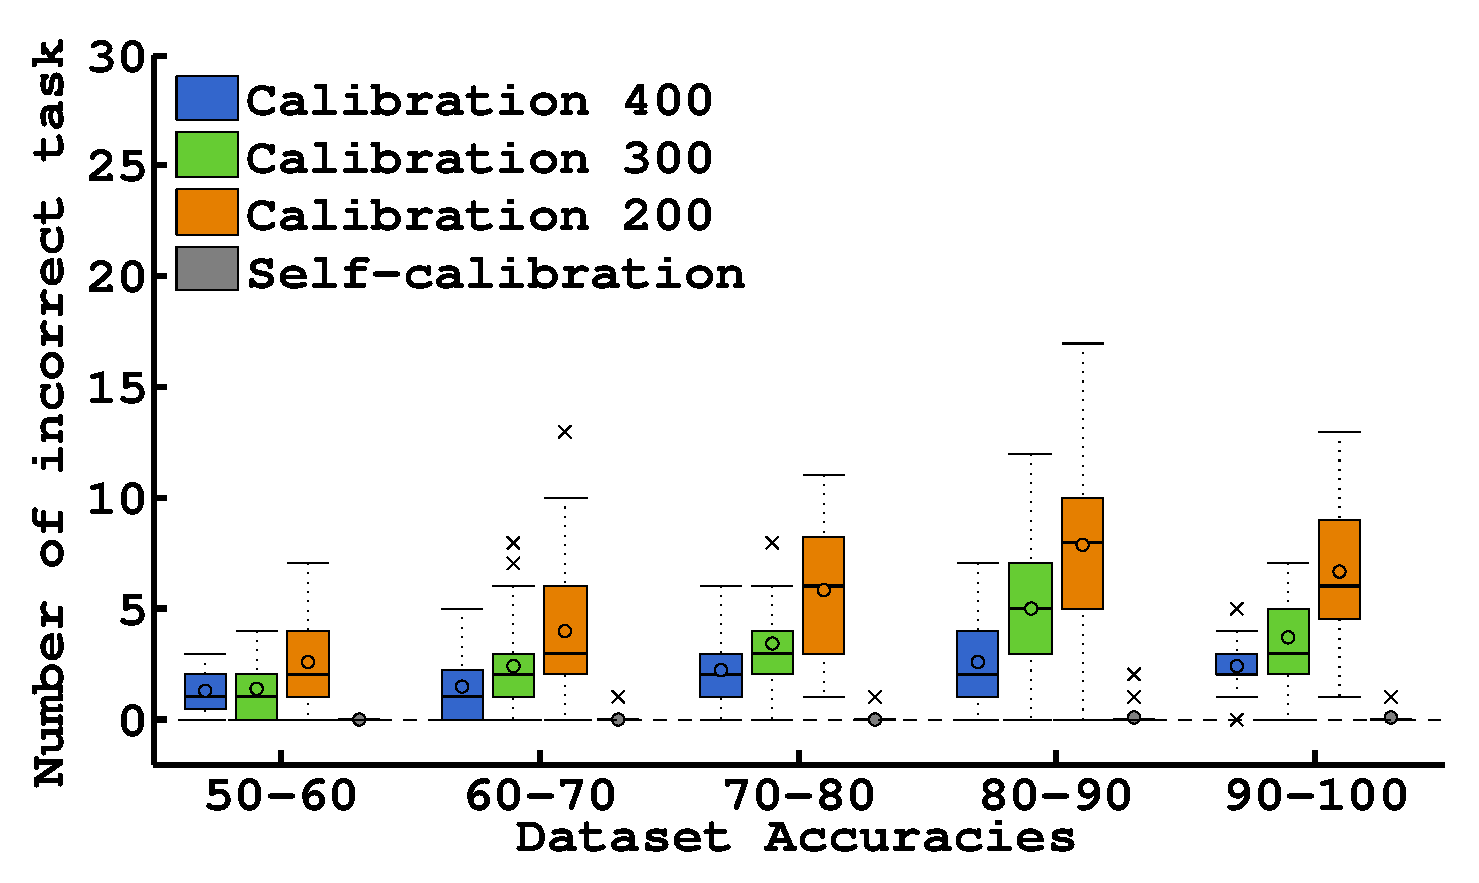
\includegraphics[width=\plotsize\columnwidth]{\imgpath/plot_EEG_calib_nWrong.eps}
\caption{Number of task incorrectly achieved in 500 steps with EEG data. Calibration methods, which do not update their models once calibrated, make more errors.}
\label{fig:nWrongEEG}
\end{figure}

\subsection{Last 100 iterations performances}

Figure~\ref{fig:nCorrectEEG_last100} compares the number of task that can be achieved during the last 100 steps with EEG data. With 80-90\% dataset quality, all methods achieve an average success rate of one task every 20 steps. However calibration methods, which do not update their models once calibrated, make more mistakes (see figure \ref{fig:nWrongEEG_last100}).

\begin{figure}[!ht]
\centering
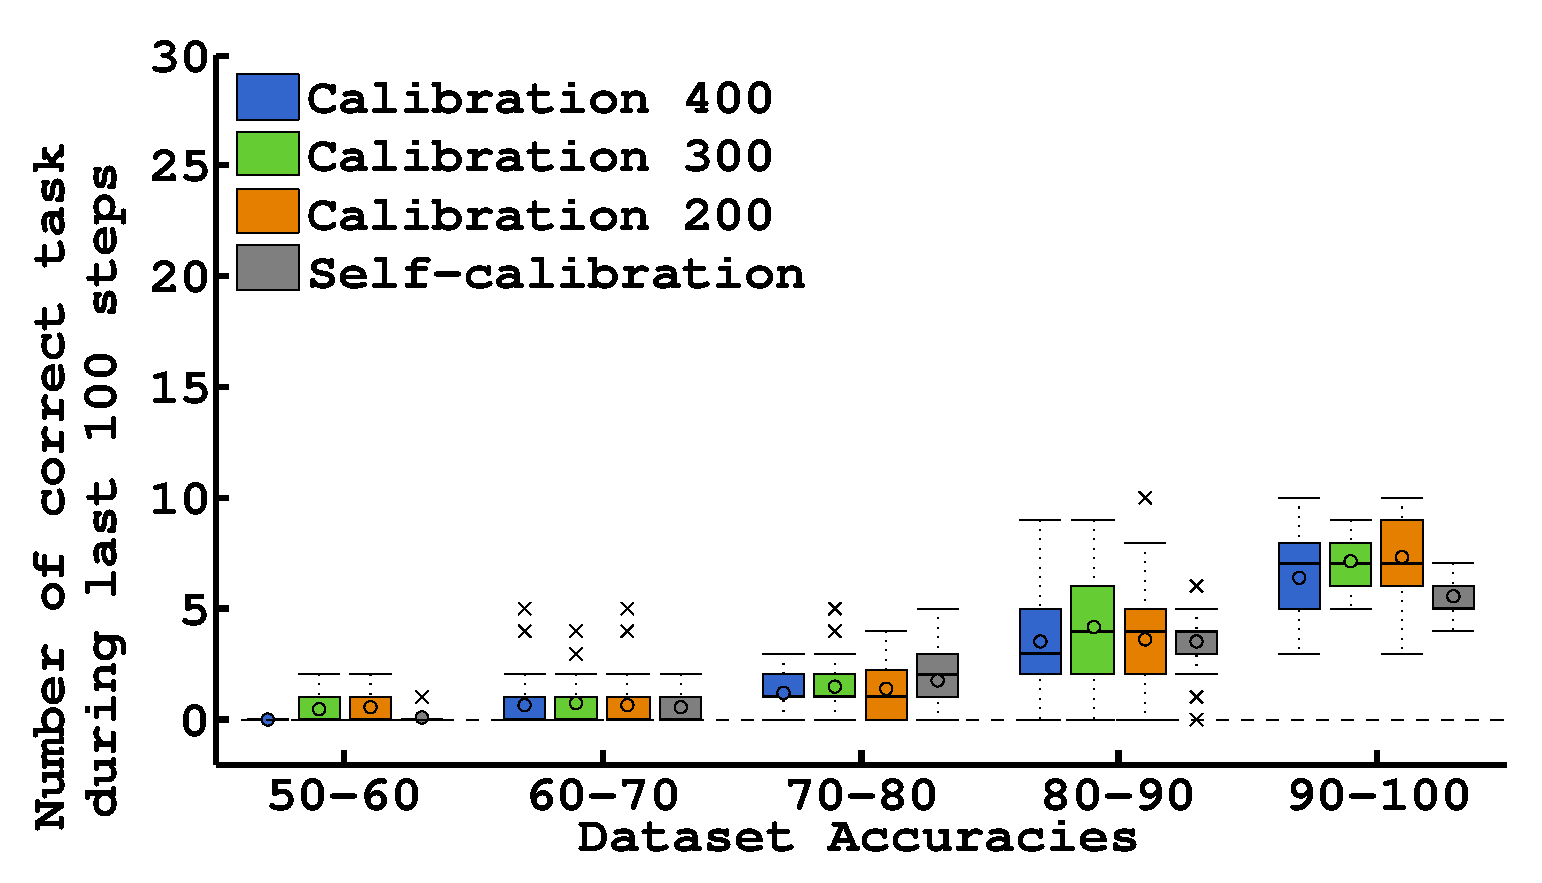
\includegraphics[width=\plotsize\columnwidth]{\imgpath/plot_EEG_calib_nCorrect_last100.eps}
\caption{Number of task correctly achieved during the last 100 steps with EEG data. All methods have equivalent successful reaching rate.}
\label{fig:nCorrectEEG_last100}
\end{figure} 

\begin{figure}[!ht]
\centering
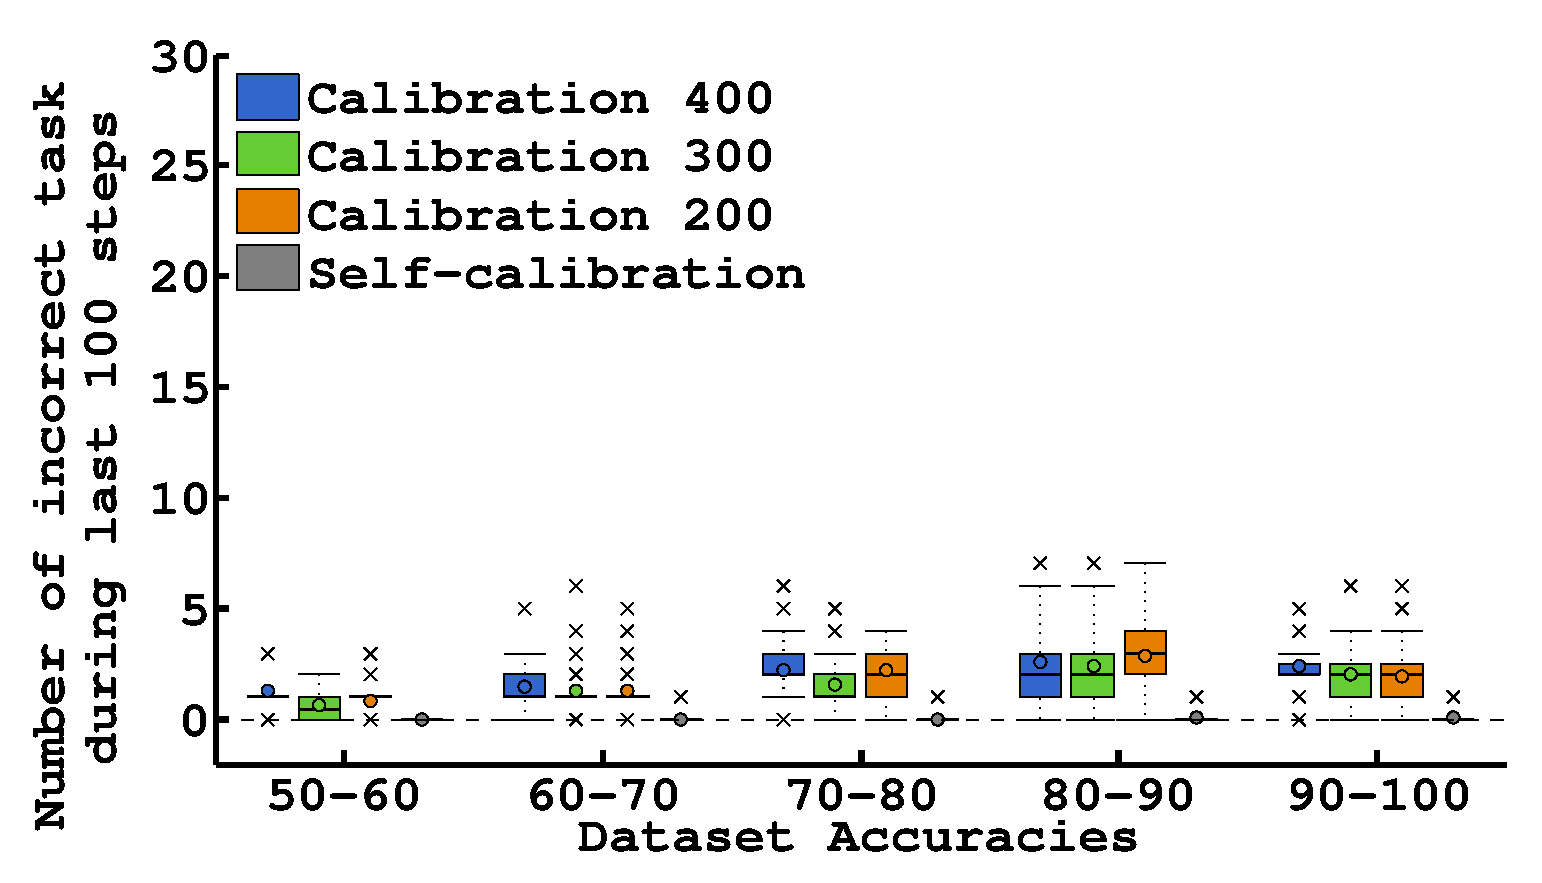
\includegraphics[width=\plotsize\columnwidth]{\imgpath/plot_EEG_calib_nWrong_last100.eps}
\caption{Number of task incorrectly achieved during the last 100 steps with EEG data. Calibration methods, which do not update their models once calibrated, make more errors.}
\label{fig:nWrongEEG_last100}
\end{figure} 

shows the number of tasks identified with respect to the accuracy of the dataset, and the number of tasks incorrectly identified. Notice how the number of identified task is correlated to the quality of the dataset. Importantly, we were able to identify 15 to 20 tasks in 500 steps on good quality dataset without the need for a calibration procedure.


%%%%%%%%%%%%%%%%%%%%%%%%%%%%%%%%%%%%%%%%%%%%%%
%%%%%%%%%%%%%%%%%%%%%%%%%%%%%%%%%%%%%%%%%%%%%%
%%%%%%%%%%%%%%%%%%%%%%%%%%%%%%%%%%%%%%%%%%%%%%
%%%%%%%%%%%%%%%%%%%%%%%%%%%%%%%%%%%%%%%%%%%%%%
%%%%%%%%%%%%%%%%%%%%%%%%%%%%%%%%%%%%%%%%%%%%%%
\section{Why we are cheating with pre-recorder EEG samples}


cite the work of chavariage and inaki which show variabliltiy in the teaching signals due to the task and teachign protocol

We can identify two main differences between our method and the usual calibration procedure for this kind of BCI experiments:
\begin{enumerate}
\item \textbf{Positive/Negative percent ratio of training examples}. Following the literature \cite{chavarriaga2010learning, iturrate2013task} we used a 80/20 percent ratio. Table \ref{tab:correctLabelRatio} shows the positive/negative ratio obtained following our planning method. The ratio we obtain is more balanced, resulting in classifiers with better properties. However a 50/50 percent ratio may lead to practical problems during online real world experiments and should be studied in more details, see open questions in section \ref{sec:conclusion}.
\item \textbf{Online update of multiple classifiers.} Our method integrates new data at every step whose label can differ between task hypothesis. For incorrect task hypothesis, the associated label can be incorrect and decrease the performance of the associated classifier, see figure \ref{fig:planningExplained}c. This dynamic can be observed in figure \ref{fig:sequence_evolution} where classifiers associated to incorrect tasks (in blue) have lower estimated accuracies than the correct one (in red). As a result our algorithm makes different predictions and updates for each hypothesis.
\end{enumerate}

\begin{table}
\centering
\begin{tabular}{c c c}
Dataset Accuracies & Self-calibration & Calibration \\ \hline
50-60 & 0.48 (0.02) & 0.8 (0) \\
60-70 & 0.50 (0.03) & 0.8 (0) \\
70-80 & 0.53 (0.03) & 0.8 (0) \\
80-90 & 0.57 (0.03) & 0.8 (0) \\
90-100 & 0.59 (0.01) & 0.8 (0) \\
\end{tabular}
\caption{Mean ratio of positive examples in training dataset (standard deviation shown in parenthesis). Calibration procedure for ErrP EEG signal usual account for a 80 percent ratio of positive examples. However when following our method we collect as many positive than negative examples. This is likely to impact the quality of Errp signal received from the human during online experiment.}
\label{tab:correctLabelRatio}
\end{table}

\begin{figure}[!ht]
\centering
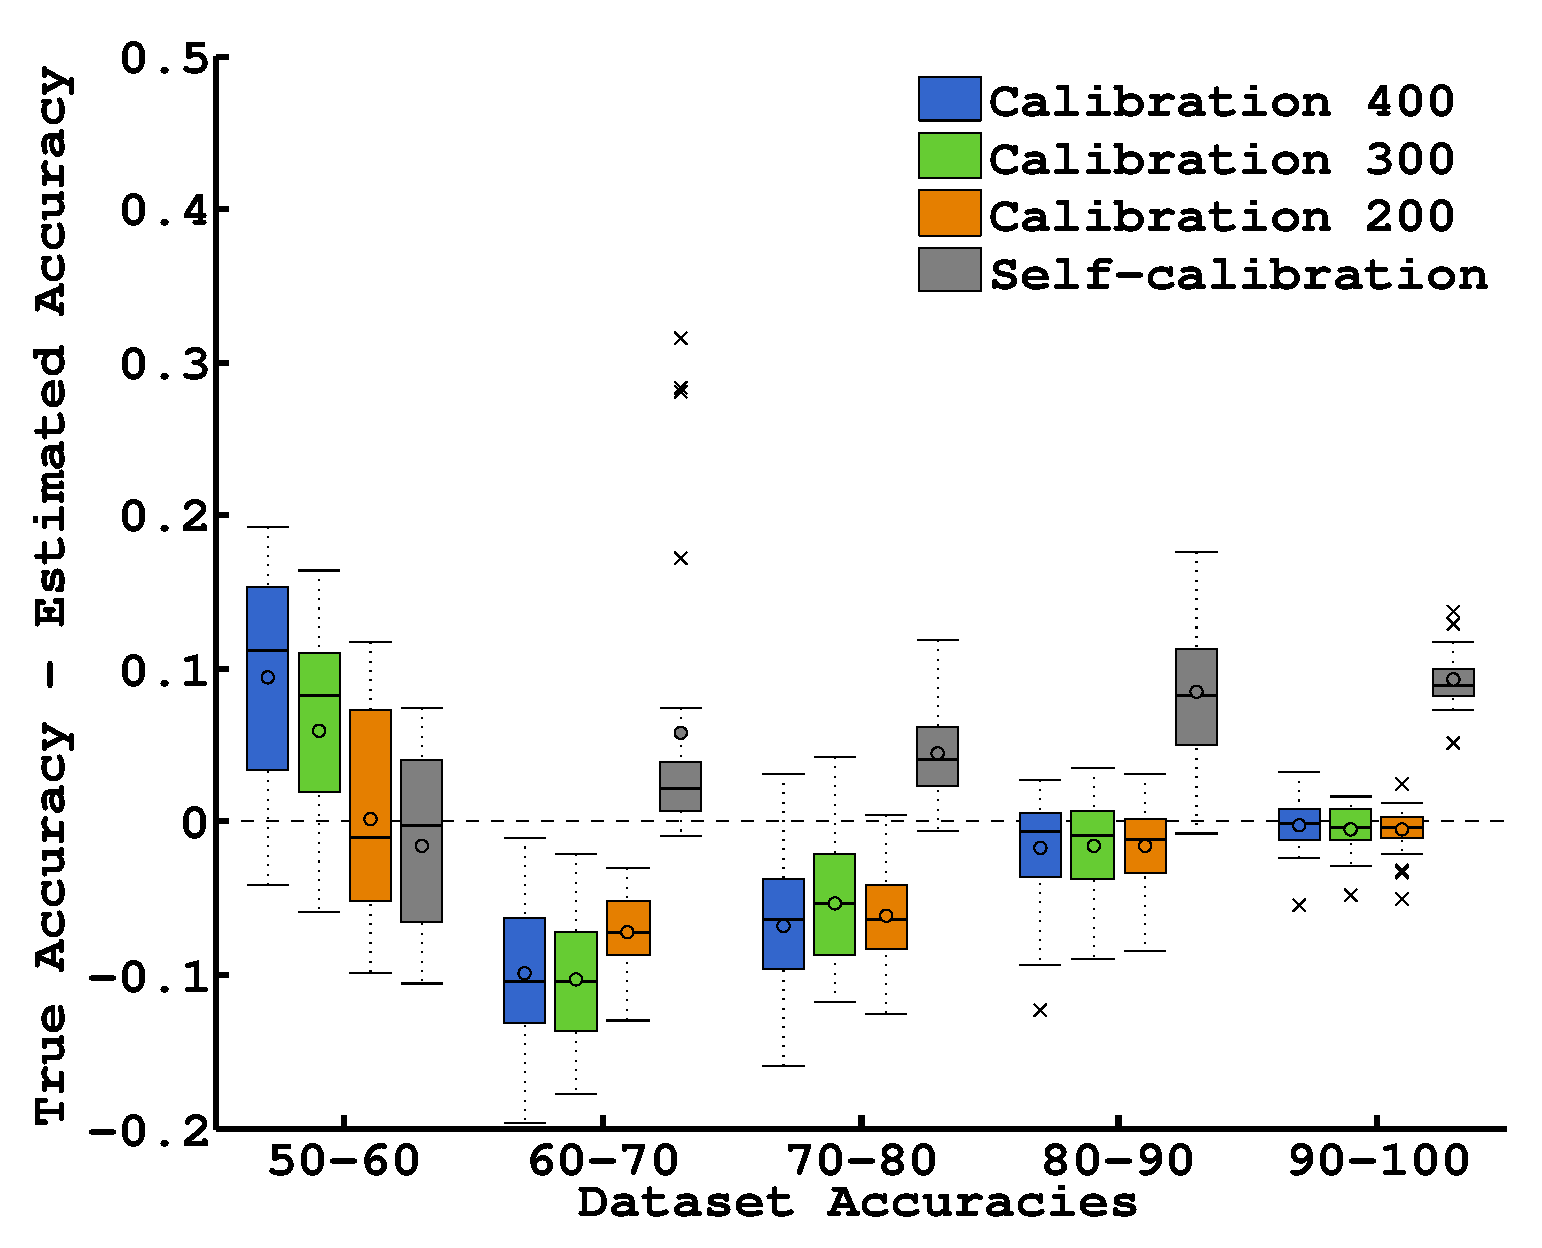
\includegraphics[width=\plotsize\columnwidth]{\imgpath/plot_explaination_for_calib_failure.eps}
\caption{Difference between true accuracy and estimated accuracy. True accuracy is the performance of the classifier on the unused data. Estimated accuracy is the 10 fold cross validation performance of the classifier on collected data. A negative(positive) value indicates the classifier is over(under)-estimating its performance. Calibration methods tend to produce over-confident classifiers, certainly due to the biased positive to negative training example ratio, see table \ref{tab:correctLabelRatio}.}
\label{fig:calibFail}
\end{figure}

%%%%%%%%%%%%%%%%%%%%%%%%%%%%%%%%%%%%%%%%%%%%%%
%%%%%%%%%%%%%%%%%%%%%%%%%%%%%%%%%%%%%%%%%%%%%%
%%%%%%%%%%%%%%%%%%%%%%%%%%%%%%%%%%%%%%%%%%%%%%
%%%%%%%%%%%%%%%%%%%%%%%%%%%%%%%%%%%%%%%%%%%%%%
%%%%%%%%%%%%%%%%%%%%%%%%%%%%%%%%%%%%%%%%%%%%%%
\section{Including Prior Information}

\begin{figure}[!ht]
\centering
\includegraphics[width=\plotsize\columnwidth]{\imgpath/powermatching/timefirst.eps}
\caption{Number of steps to complete first task with EEG data. Comparison between our general method (matching), or using the information that ``incorrect'' signals are more powerful than the ``correct'' (power), or both method combined (power matching). The use of the power information affect the usual performance for the low quality dataset. For datasets of low quality, while the time to first seems more advantageous for the method using the power information, most of the estimated task are erroneous (see Figure~\ref{fig:errorfirst_powermatching}) which makes the use of the power information critical for such low quality data. However those errors occurs for very low quality datasets, which are not the main target of our algorithm. For the datasets of higher quality, the power information allow to slightly speed up the learning compared to our method (matching) which do not rely on known information.}
\label{fig:timefirst_powermatching}
\end{figure} 


\begin{figure}[!ht]
\centering
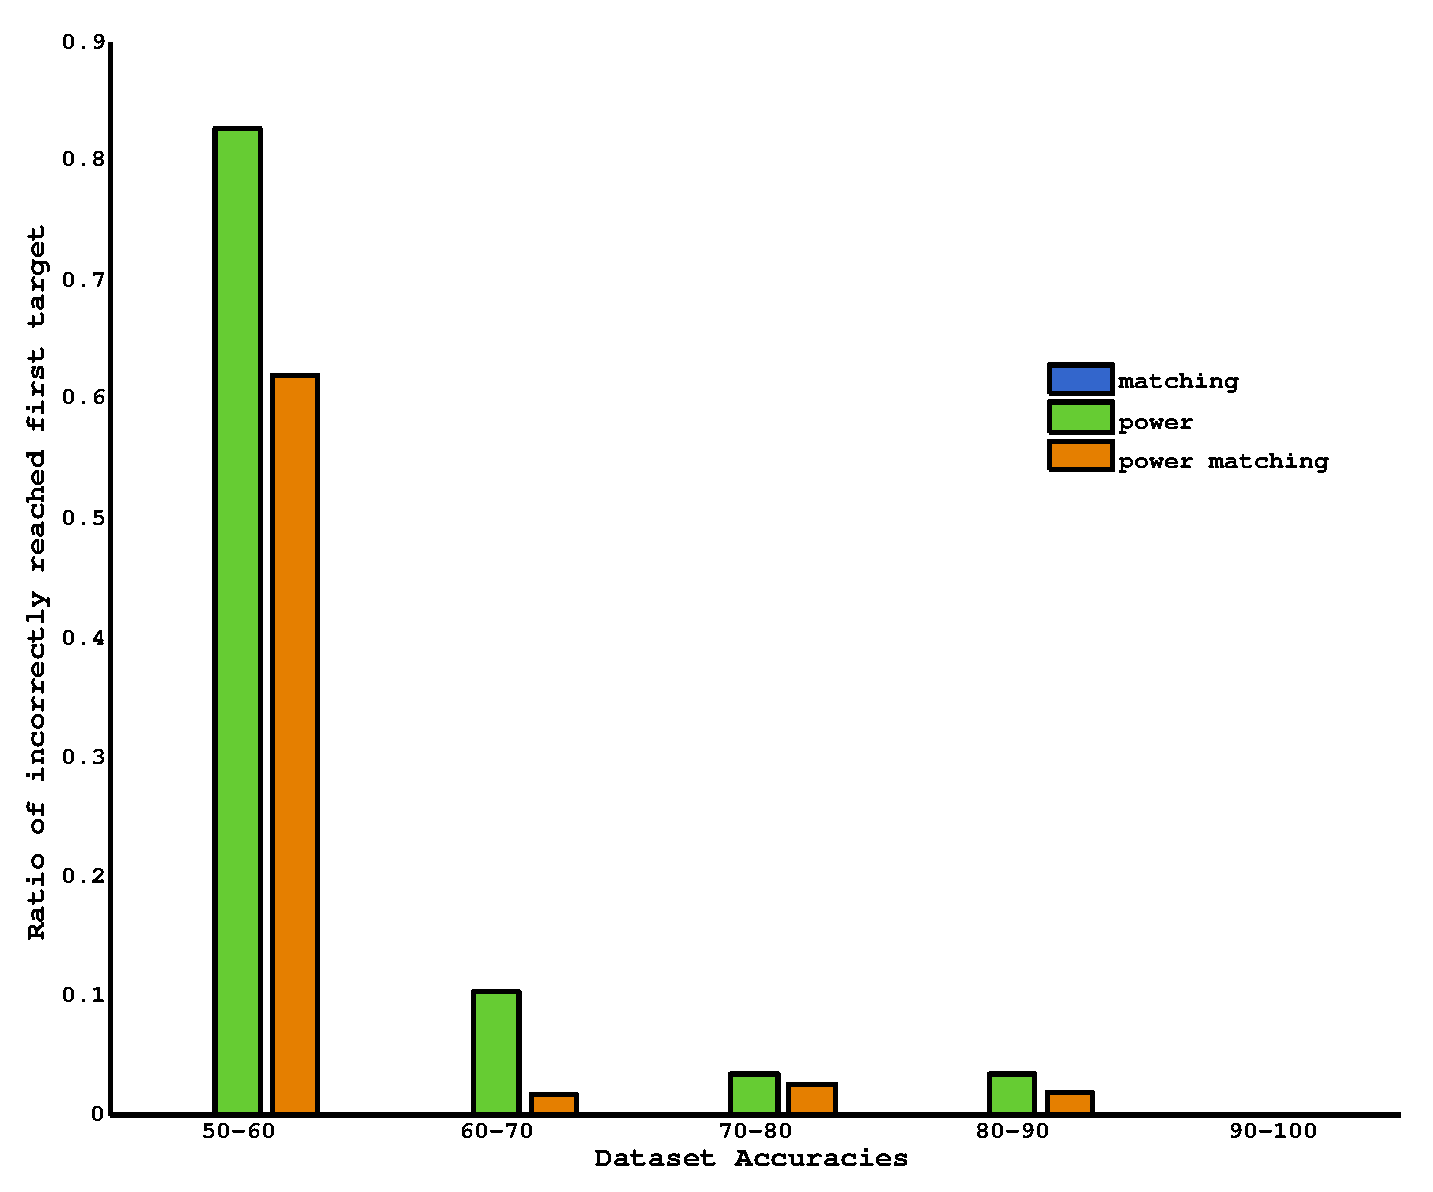
\includegraphics[width=\plotsize\columnwidth]{\imgpath/powermatching/errorfirst.eps}
\caption{Percentage of time the first task estimated was erroneous using EEG data. Comparison between our general method (matching), or using the information that ``incorrect'' signals are more powerful than the ``correct'' (power), or both method combined (power matching). For low quality datasets, the power information increases the number of erroneous estimation. However those errors occurs for very low quality datasets, which are not the main target of our algorithm.}
\label{fig:errorfirst_powermatching}
\end{figure} 


\begin{figure}[!ht]
\centering
\includegraphics[width=\plotsize\columnwidth]{\imgpath/powermatching/correct.eps}
\caption{Number of task correctly achieved in 500 steps with EEG data. Comparison between our general method (matching), or using the information that ``incorrect'' signals are more powerful than the ``correct'' (power), or both method combined (power matching). The power information alone is sufficient to solve our problem but is less efficient than the other methods.}
\label{fig:nCorrect_powermatching}
\end{figure} 

\begin{figure}[!ht]
\centering
\includegraphics[width=\plotsize\columnwidth]{\imgpath/powermatching/error.eps}
\caption{Number of task correctly achieved in 500 steps with EEG data. Comparison between our general method (matching), or using the information that ``incorrect'' signals are more powerful than the ``correct'' (power), or both method combined (power matching). The power information makes more mistakes for low quality dataset which also impact the power matching method. However those errors occurs for very low quality datasets, which are not the main target of our algorithm.}
\label{fig:nWrongEEG_powermatching}
\end{figure} 

For such data it would be better to change the representation of the signal or the classifier used in order to get better .


\begin{figure}[!ht]
\centering
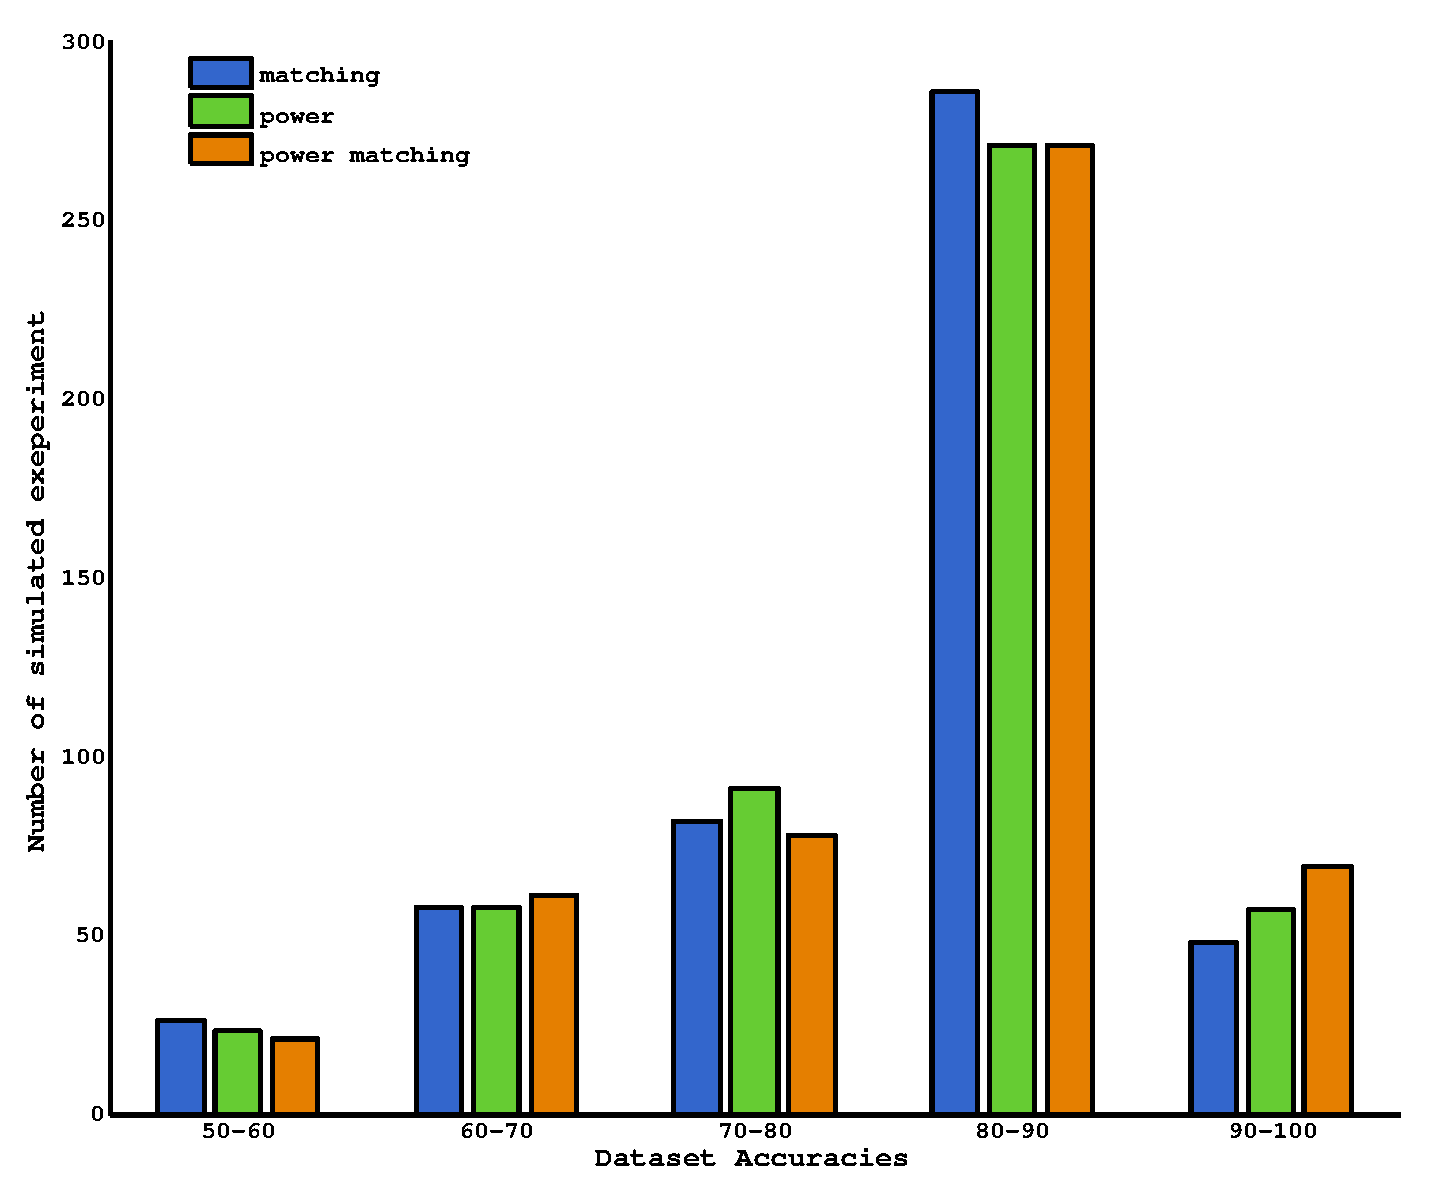
\includegraphics[width=\plotsize\columnwidth]{\imgpath/powermatching/nSim.eps}
\caption{\todo{use a table instead of this figure}}
\label{fig:nSim_powermatching}
\end{figure} 


%%%%%%%%%%%%%%%%%%%%%%%%%%%%%%%%%%%%%%%%%%%%%%
%%%%%%%%%%%%%%%%%%%%%%%%%%%%%%%%%%%%%%%%%%%%%%
%%%%%%%%%%%%%%%%%%%%%%%%%%%%%%%%%%%%%%%%%%%%%%
%%%%%%%%%%%%%%%%%%%%%%%%%%%%%%%%%%%%%%%%%%%%%%
%%%%%%%%%%%%%%%%%%%%%%%%%%%%%%%%%%%%%%%%%%%%%%
\section{Experiments with real users}

\begin{figure}[!ht]
\centering
\includegraphics[width=\plotsize\columnwidth]{\imgpath/onlineXP/timefirst.eps}
\caption{Number of steps to complete first task for all subjects in our online experiments. The results are plotted against the a posteriori computed 10 fold accuracy of our classifier on each subject EEG signals. The relation between data quality and the time to first task is in line with our simulated results shown in Figure~\ref{fig:timefirst_powermatching} Note that this first target was always the correct one for every subject.}
\label{fig:timefirst_online}
\end{figure} 


\begin{figure}[!ht]
\centering
\includegraphics[width=\plotsize\columnwidth]{\imgpath/onlineXP/correct.eps}
\caption{a}
\label{fig:correct_online}
\end{figure} 

\begin{figure}[!ht]
\centering
\includegraphics[width=\plotsize\columnwidth]{\imgpath/onlineXP/error.eps}
\caption{a}
\label{fig:error_online}
\end{figure} 

\todo{summarize all this in a table, but keep two figure to have a visuals which is important.}

\transition

\todo{recap}

Those results with real EEG signals allow us to believe such algorithm could have practical application into the real word. By removing the user of an expert to collect and calibrate the system, we may democratize the use of brain computer interface and allow their users to go out of the labs. However there is number of limitation that would need to be addressed, such as the synchronous interactions assumption, the discrete state, discrete action. Most of the current limitation of this work will be addressed in the next section.

\todo{list limitation here}
